\documentclass[11pt,a4paper]{article}

% ==================== TEMEL PAKETLER (pdflatex) ====================
\usepackage[T1]{fontenc}
\usepackage[utf8]{inputenc}
\usepackage{lmodern}
\usepackage[a4paper,margin=2cm,top=2.4cm,bottom=2.4cm]{geometry}
\usepackage{xcolor}
\usepackage{colortbl}
\usepackage{array}
\usepackage{booktabs}
\usepackage{tabularx}
\usepackage{amsmath}
\usepackage{amssymb}
\usepackage{fancyhdr}
\usepackage{tikz}
\usetikzlibrary{arrows.meta,calc,patterns}
\usepackage{hyperref}

% ==================== RENK PALETİ ====================
\definecolor{anaMavi}{HTML}{1B3A5B}
\definecolor{vurguMavi}{HTML}{2E6DA4}
\definecolor{acikMavi}{HTML}{EAF2F9}
\definecolor{turuncu}{HTML}{D9701E}
\definecolor{yesil}{HTML}{2E7D32}
\definecolor{acikYesil}{HTML}{E8F5E9}
\definecolor{kirmizi}{HTML}{C0392B}
\definecolor{mor}{HTML}{6C3483}
\definecolor{acikMor}{HTML}{F3E9F7}
\definecolor{acikGri}{HTML}{F4F5F7}
\definecolor{ortaGri}{HTML}{6B7280}
\definecolor{koyuGri}{HTML}{2D2D2D}
\definecolor{grafikMavi}{HTML}{2E6DA4}

% ==================== HYPERREF ====================
\hypersetup{
  colorlinks=true,
  linkcolor={[HTML]{2E6DA4}},
  urlcolor={[HTML]{2E6DA4}},
  pdftitle={Kalkülüs: Limit, Türev ve İntegral Rehberi},
  pdfauthor={Kalkülüs Rehberi},
  bookmarksnumbered=true
}

% ==================== BAŞLIK STİLLERİ ====================
\setcounter{secnumdepth}{0}
\newcounter{secc}
\newcounter{subsecc}[secc]
\newcommand{\gsec}[1]{\par\phantomsection\stepcounter{secc}%
  \setcounter{subsecc}{0}%
  \vspace{18pt}{\color{anaMavi}\Large\bfseries\thesecc.\hspace{0.5em}#1}\par
  \vspace{2pt}{\color{turuncu}\rule{\linewidth}{1.6pt}}\par\vspace{8pt}%
  \addcontentsline{toc}{section}{\protect\numberline{\thesecc}#1}\markboth{#1}{#1}}
\newcommand{\gsub}[1]{\par\phantomsection\stepcounter{subsecc}%
  \vspace{11pt}{\color{vurguMavi}\large\bfseries\thesecc.\thesubsecc\hspace{0.5em}#1}\par\vspace{4pt}%
  \addcontentsline{toc}{subsection}{\protect\numberline{\thesecc.\thesubsecc}#1}}
\newcommand{\gsubsub}[1]{\par\vspace{7pt}{\color{koyuGri}\normalsize\bfseries #1}\par\vspace{2pt}}

% Kısım (Part) başlığı
\newcommand{\gpart}[2]{\clearpage
  \begin{center}\vspace*{1.5cm}
  {\color{turuncu}\rule{0.7\linewidth}{1.5pt}}\\[10pt]
  {\color{ortaGri}\Large KISIM #1}\\[8pt]
  {\color{anaMavi}\Huge\bfseries #2}\\[10pt]
  {\color{turuncu}\rule{0.7\linewidth}{1.5pt}}
  \end{center}\vspace{1cm}}

% ==================== BAŞLIK / ALTBİLGİ ====================
\setlength{\headheight}{14pt}
\pagestyle{fancy}
\fancyhf{}
\renewcommand{\headrulewidth}{0.4pt}
\renewcommand{\footrulewidth}{0.4pt}
\fancyhead[L]{\small\color{ortaGri}Kalkülüs: Limit, Türev, İntegral}
\fancyhead[R]{\small\color{ortaGri}\leftmark}
\fancyfoot[C]{\small\color{ortaGri}\thepage}

% ==================== ÖZEL KUTULAR ====================
\newcommand{\callout}[4]{\par\smallskip\noindent\begingroup
  \setlength{\fboxsep}{8pt}\setlength{\fboxrule}{0.8pt}%
  \fcolorbox{#1}{#2}{\parbox{\dimexpr\linewidth-2\fboxsep-2\fboxrule\relax}{%
    {\bfseries\color{#1}#3}\par\smallskip #4}}\endgroup\par\smallskip}
\newcommand{\bilgi}[1]{\callout{vurguMavi}{acikMavi}{Bilgi}{#1}}
\newcommand{\ipucu}[1]{\callout{yesil}{acikYesil}{İpucu}{#1}}
\newcommand{\uyari}[1]{\callout{kirmizi}{kirmizi!7}{Dikkat}{#1}}
\newcommand{\tanim}[2][Tanım]{\callout{vurguMavi}{acikMavi}{#1}{#2}}
\newcommand{\kural}[2][Kural]{\callout{mor}{acikMor}{#1}{#2}}
\newcommand{\notk}[2][Not]{\callout{mor}{acikMor}{#1}{#2}}
\newcommand{\ornek}[2][Örnek]{\callout{ortaGri!90!black}{acikGri}{#1}{#2}}

% Soru / Çözüm sistemi
\newcounter{soruc}
\newcommand{\soru}[1]{\par\smallskip\refstepcounter{soruc}%
  \noindent\begingroup\setlength{\fboxsep}{8pt}\setlength{\fboxrule}{0.8pt}%
  \fcolorbox{turuncu}{turuncu!6}{\parbox{\dimexpr\linewidth-2\fboxsep-2\fboxrule\relax}{%
  {\bfseries\color{turuncu}Soru \thesoruc}\par\smallskip #1}}\endgroup\par\smallskip}
\newcommand{\cozum}{\par\noindent{\bfseries\color{yesil}Çözüm.}\ }

% Yardımcı komutlar
\newcommand{\code}[1]{\texttt{\color{koyuGri}#1}}
\renewcommand{\arraystretch}{1.35}
\newcommand{\lm}[2]{\lim_{#1 \to #2}}

% ==================== BAŞLANGIÇ ====================
\begin{document}

% ---------- KAPAK ----------
\begin{titlepage}
\centering
\vspace*{1.4cm}
{\color{turuncu}\rule{\textwidth}{2pt}}\\[8pt]
{\color{anaMavi}\Huge\bfseries Kalkülüs}\\[10pt]
{\color{vurguMavi}\LARGE Limit, Türev ve İntegral Rehberi}\\[8pt]
{\color{ortaGri}\large Bol Çözümlü Soru ve Grafiklerle Anlatım}\\[6pt]
{\color{turuncu}\rule{\textwidth}{2pt}}\\[1.4cm]

\begin{center}
\fcolorbox{vurguMavi}{acikMavi}{\parbox{0.86\textwidth}{\centering\large
Bu belge kalkülüsün üç temel konusunu --- \textbf{limit, türev (derivative) ve
integral} --- sıfırdan, \textbf{grafiklerle} ve \textbf{bol çözümlü soruyla}
anlatır. Her kavram önce sezgisel olarak, sonra kurallarıyla verilir; ardından
farklı soru tipleri adım adım çözülür.\vspace{4pt}}}
\end{center}

\vspace{0.8cm}
\begin{center}
\fcolorbox{ortaGri!50}{acikGri}{\parbox{0.86\textwidth}{\small
\textbf{Kısım 1 --- Limit:} limit kavramı \& grafik yorumu \textbullet\ tek
taraflı limitler \textbullet\ limit hesaplama teknikleri \textbullet\ belirsizlik
(\code{0/0}) \textbullet\ trigonometrik limitler \textbullet\ süreklilik
(continuity) \textbullet\ sonsuzda limit \& asimptotlar.\vspace{4pt}

\textbf{Kısım 2 --- Türev (Derivative):} türev tanımı \& teğet doğru
\textbullet\ türev kuralları (power, product, quotient, chain) \textbullet\
trigonometrik, üstel, logaritmik türevler \textbullet\ kapalı türev
\textbullet\ maksimum-minimum \textbullet\ optimizasyon \textbullet\ L'Hôpital.\vspace{4pt}

\textbf{Kısım 3 --- İntegral:} belirsiz integral (antiderivative) \textbullet\
integral teknikleri (substitution, by parts, kısmi kesir) \textbullet\ belirli
integral \& Riemann toplamı \textbullet\ Kalkülüsün Temel Teoremi \textbullet\
alan \& dönel hacim.\vspace{4pt}}}
\end{center}

\vfill
{\color{ortaGri}\large Hazırlanma Tarihi: 13 Temmuz 2026}\\[4pt]
{\color{ortaGri} Terimler İngilizce \textbullet\ Anlatım Türkçe \textbullet\ Grafiklerle}
\vspace*{0.6cm}
\end{titlepage}

% ---------- İÇİNDEKİLER ----------
\tableofcontents
\thispagestyle{empty}
\clearpage

% #####################################################################
\gpart{1}{Limit}
% #####################################################################

% =====================================================================
\gsec{Limit Kavramı}
% =====================================================================

Limit, kalkülüsün temel taşıdır; hem türev hem integral limit üzerine
kuruludur. Sezgisel olarak limit şu soruyu sorar: ``$x$ bir $a$ değerine
\emph{yaklaşırken}, $f(x)$ hangi değere \emph{yaklaşır}?'' Dikkat: soru
``$f(a)$ nedir?'' değildir --- limit, fonksiyonun o noktadaki değeriyle değil,
\emph{yakınındaki} davranışıyla ilgilenir.

\gsub{Sezgisel Tanım ve Gösterim}

\tanim{$x$, $a$'ya yaklaşırken $f(x)$ değeri $L$ sayısına istenildiği kadar
yaklaşıyorsa, $f$'nin $a$ noktasındaki \emph{limiti} $L$'dir ve şöyle yazılır:
\[
\lim_{x \to a} f(x) = L .
\]}

Aşağıdaki grafikte $f(x)=x^2$ fonksiyonu için $x \to 2$ iken $f(x) \to 4$
olduğunu görüyoruz. $x$ soldan (1.9, 1.99\dots) ve sağdan (2.1, 2.01\dots)
yaklaşırken fonksiyon değerleri hep $4$'e yaklaşır.

\begin{center}
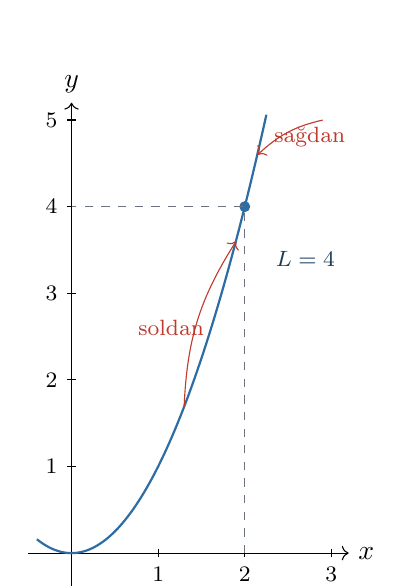
\begin{tikzpicture}[scale=1.1]
\draw[->] (-0.5,0)--(3.2,0) node[right]{$x$};
\draw[->] (0,-0.5)--(0,5.2) node[above]{$y$};
\foreach \x in {1,2,3} \draw (\x,0.05)--(\x,-0.05) node[below]{\footnotesize\x};
\foreach \y in {1,2,3,4,5} \draw (0.05,\y)--(-0.05,\y) node[left]{\footnotesize\y};
\draw[grafikMavi,thick,domain=-0.4:2.25,samples=100] plot (\x,{\x*\x});
\filldraw[grafikMavi] (2,4) circle (1.6pt);
\draw[dashed,ortaGri] (2,0)--(2,4)--(0,4);
\draw[->,kirmizi] (1.3,1.69) to[bend left=15] (1.9,3.6);
\draw[->,kirmizi] (2.9,5) to[bend right=15] (2.15,4.6);
\node[kirmizi] at (1.15,2.6) {\footnotesize soldan};
\node[kirmizi] at (2.75,4.8) {\footnotesize sağdan};
\node[anaMavi] at (2.7,3.4) {\footnotesize $L=4$};
\end{tikzpicture}
\end{center}

\gsub{Tek Taraflı Limitler (One-Sided Limits)}

Bazen fonksiyon, bir noktaya soldan ve sağdan \emph{farklı} değerlerle
yaklaşır. Bu durumda tek taraflı limitleri ayrı ayrı yazarız:
\[
\lim_{x \to a^-} f(x) \quad(\text{soldan limit}), \qquad
\lim_{x \to a^+} f(x) \quad(\text{sağdan limit}).
\]

\kural[Limitin Varlığı]{Bir noktadaki (iki taraflı) limitin \emph{var olması}
için, soldan ve sağdan limitlerin \textbf{eşit} olması gerekir:
\[
\lim_{x \to a} f(x) = L \quad\Longleftrightarrow\quad
\lim_{x \to a^-} f(x) = \lim_{x \to a^+} f(x) = L .
\]
Eşit değillerse limit \emph{yoktur} (does not exist, DNE).}

Aşağıdaki parçalı fonksiyonda $x=1$'de bir \emph{sıçrama} (jump) vardır:
soldan limit $1$, sağdan limit $3$'tür. Eşit olmadıklarından $x=1$'de limit
yoktur.

\begin{center}
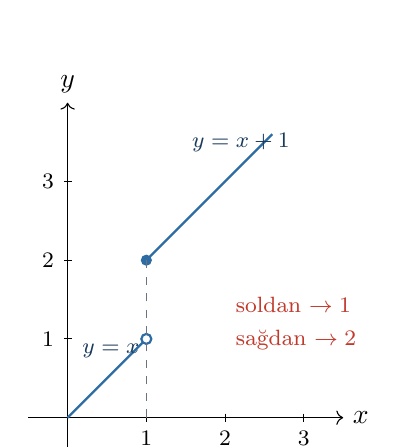
\begin{tikzpicture}[scale=1.0]
\draw[->] (-0.5,0)--(3.5,0) node[right]{$x$};
\draw[->] (0,-0.5)--(0,4) node[above]{$y$};
\foreach \x in {1,2,3} \draw (\x,0.05)--(\x,-0.05) node[below]{\footnotesize\x};
\foreach \y in {1,2,3} \draw (0.05,\y)--(-0.05,\y) node[left]{\footnotesize\y};
% soldan parça: y = x, x<1
\draw[grafikMavi,thick,domain=0:1] plot (\x,{\x});
\filldraw[white,draw=grafikMavi,thick] (1,1) circle (1.8pt); % açık uç
% sağdan parça: y = x+1, x>=1  (1'de 2? yapalım jump 3)
\draw[grafikMavi,thick,domain=1:2.6] plot (\x,{\x+1});
\filldraw[grafikMavi] (1,2) circle (1.8pt); % kapalı uç
\draw[dashed,ortaGri] (1,0)--(1,2);
\node[anaMavi] at (0.55,0.85) {\footnotesize $y=x$};
\node[anaMavi] at (2.2,3.5) {\footnotesize $y=x+1$};
\node[kirmizi,align=left] at (2.9,1.2) {\footnotesize soldan $\to 1$\\ \footnotesize sağdan $\to 2$};
\end{tikzpicture}
\end{center}

\notk[Parçalı fonksiyon örneği]{Yukarıdaki grafik şu fonksiyona aittir:
$f(x)=x$ (eğer $x<1$) ve $f(x)=x+1$ (eğer $x\ge 1$). Soldan limit
$\lim_{x\to1^-}f(x)=1$, sağdan limit $\lim_{x\to1^+}f(x)=2$. Bunlar farklı
olduğu için $\lim_{x\to1}f(x)$ \textbf{yoktur}, ama fonksiyon $x=1$'de
tanımlıdır ($f(1)=2$).}

\gsub{Limit Kuralları (Limit Laws)}

Limitler, aşağıdaki kurallarla parça parça hesaplanabilir. $\lm{x}{a}f(x)=L$
ve $\lm{x}{a}g(x)=M$ olsun:

\begin{center}
\begin{tabularx}{\textwidth}{@{}>{\bfseries\color{anaMavi}}l >{$}l<{$} @{}}
\toprule
\rowcolor{acikMavi}\color{anaMavi}\textbf{Kural} & \color{anaMavi}\textbf{Formül}\\
\midrule
Toplam / fark & \lm{x}{a}[f(x)\pm g(x)] = L \pm M\\
\rowcolor{acikGri} Sabit katı & \lm{x}{a}[c\cdot f(x)] = c\,L\\
Çarpım & \lm{x}{a}[f(x)g(x)] = L\cdot M\\
\rowcolor{acikGri} Bölüm & \lm{x}{a}\dfrac{f(x)}{g(x)} = \dfrac{L}{M}\ \ (M\ne 0)\\
Kuvvet & \lm{x}{a}[f(x)]^n = L^n\\
\bottomrule
\end{tabularx}
\end{center}

\soru{$\displaystyle \lim_{x \to 3}\,(x^2 - 2x + 5)$ limitini hesaplayın.}

\cozum Polinomlar her yerde süreklidir; bu yüzden limit, doğrudan yerine koyma
(direct substitution) ile bulunur:
\[
\lim_{x \to 3}(x^2 - 2x + 5) = 3^2 - 2\cdot 3 + 5 = 9 - 6 + 5 = 8 .
\]

\soru{$\displaystyle \lim_{x \to 2}\frac{x + 1}{x - 5}$ limitini hesaplayın.}

\cozum Payda $x=2$'de sıfır olmadığından ($2-5=-3\ne 0$) yine yerine koyarız:
\[
\lim_{x \to 2}\frac{x+1}{x-5} = \frac{2+1}{2-5} = \frac{3}{-3} = -1 .
\]

% =====================================================================
\gsec{Limit Hesaplama Teknikleri}
% =====================================================================

Doğrudan yerine koyma her zaman işe yaramaz. En sık karşılaşılan durum,
yerine koyunca $\frac{0}{0}$ biçiminde bir \emph{belirsizlik}
(indeterminate form) elde etmektir. Bu, ``limit yok'' demek değildir ---
ifadeyi sadeleştirmek gerektiği anlamına gelir.

\uyari{$\frac{0}{0}$ bir \emph{belirsizlik biçimidir}; değeri $0$, $1$,
$\infty$ veya herhangi bir sayı olabilir. Bunu görünce panik yapma: pay ve
paydayı çarpanlara ayırıp sadeleştirerek, kök varsa eşleniğiyle çarparak
belirsizliği kaldırırsın. Diğer belirsizlik biçimleri:
$\frac{\infty}{\infty}$, $0\cdot\infty$, $\infty-\infty$.}

\gsub{Teknik 1: Çarpanlara Ayırma (Factoring)}

\soru{$\displaystyle \lim_{x \to 2}\frac{x^2 - 4}{x - 2}$ limitini hesaplayın.}

\cozum Yerine koyunca $\frac{4-4}{2-2}=\frac{0}{0}$ (belirsiz). Payı çarpanlara
ayırırız: $x^2-4=(x-2)(x+2)$. Sonra $x\ne 2$ için $(x-2)$ sadeleşir:
\[
\lim_{x\to2}\frac{(x-2)(x+2)}{x-2} = \lim_{x\to2}(x+2) = 2+2 = 4 .
\]
Grafik olarak: fonksiyon $x=2$ dışında $y=x+2$ ile aynıdır; $x=2$'de bir
\emph{delik} (removable discontinuity) vardır ama limit yine $4$'tür.

\begin{center}
\begin{tikzpicture}[scale=0.9]
\draw[->] (-0.5,0)--(4,0) node[right]{$x$};
\draw[->] (0,-0.5)--(0,5.5) node[above]{$y$};
\foreach \x in {1,2,3} \draw (\x,0.05)--(\x,-0.05) node[below]{\footnotesize\x};
\foreach \y in {2,4} \draw (0.05,\y)--(-0.05,\y) node[left]{\footnotesize\y};
\draw[grafikMavi,thick,domain=-0.3:3.3] plot (\x,{\x+2});
\filldraw[white,draw=grafikMavi,thick] (2,4) circle (1.8pt); % delik
\draw[dashed,ortaGri] (2,0)--(2,4)--(0,4);
\node[anaMavi] at (3.0,4.4) {\footnotesize $y=x+2$};
\node[kirmizi] at (2.55,3.2) {\footnotesize delik};
\end{tikzpicture}
\end{center}

\soru{$\displaystyle \lim_{x \to 3}\frac{x^2 - 9}{x^2 - 5x + 6}$ limitini
hesaplayın.}

\cozum $\frac{0}{0}$ belirsizliği. Hem payı hem paydayı çarpanlara ayırırız:
$x^2-9=(x-3)(x+3)$ ve $x^2-5x+6=(x-3)(x-2)$.
\[
\lim_{x\to3}\frac{(x-3)(x+3)}{(x-3)(x-2)}
= \lim_{x\to3}\frac{x+3}{x-2} = \frac{3+3}{3-2} = \frac{6}{1} = 6 .
\]

\gsub{Teknik 2: Eşlenikle Çarpma (Rationalizing)}

Kök içeren ifadelerde $\frac{0}{0}$ çıkarsa, pay veya paydayı \emph{eşleniğiyle}
(conjugate) çarparız.

\soru{$\displaystyle \lim_{x \to 0}\frac{\sqrt{x+4} - 2}{x}$ limitini
hesaplayın.}

\cozum $\frac{0}{0}$ belirsizliği. Payın eşleniği $\sqrt{x+4}+2$ ile pay ve
paydayı çarparız:
\[
\frac{\sqrt{x+4}-2}{x}\cdot\frac{\sqrt{x+4}+2}{\sqrt{x+4}+2}
= \frac{(x+4)-4}{x(\sqrt{x+4}+2)} = \frac{x}{x(\sqrt{x+4}+2)}
= \frac{1}{\sqrt{x+4}+2}.
\]
Şimdi yerine koyabiliriz:
\[
\lim_{x\to0}\frac{1}{\sqrt{x+4}+2} = \frac{1}{\sqrt{4}+2} = \frac{1}{4}.
\]

\gsub{Teknik 3: Ortak Payda ile Sadeleştirme}

\soru{$\displaystyle \lim_{x \to 0}\frac{\frac{1}{x+2}-\frac{1}{2}}{x}$
limitini hesaplayın.}

\cozum Paydaki iki kesri ortak paydada birleştiririz:
\[
\frac{1}{x+2}-\frac{1}{2} = \frac{2-(x+2)}{2(x+2)} = \frac{-x}{2(x+2)}.
\]
Bunu $x$'e böleriz (yani $\frac{1}{x}$ ile çarparız):
\[
\lim_{x\to0}\frac{-x}{2(x+2)}\cdot\frac{1}{x}
= \lim_{x\to0}\frac{-1}{2(x+2)} = \frac{-1}{2\cdot 2} = -\frac{1}{4}.
\]

\ipucu{\textbf{Strateji özeti:} Bir limitte önce \emph{doğrudan yerine koy}.
Sonuç bir sayıysa iş biter. $\frac{0}{0}$ çıkarsa: polinom varsa
\emph{çarpanlara ayır}, kök varsa \emph{eşlenikle çarp}, kesir içinde kesir
varsa \emph{ortak paydada birleştir}. Bir sabiti sıfıra bölüyorsan (ör.
$\frac{3}{0}$) limit sonsuz olabilir --- tek taraflı işaretlere bak.}

% =====================================================================
\gsec{Trigonometrik Limitler ve Sıkıştırma Teoremi}
% =====================================================================

Trigonometrik fonksiyonların limitlerinde çoğu zaman iki temel özdeşlik
işimizi görür. Bunlar, ileride $\sin x$ ve $\cos x$'in türevlerini türetirken
de kullanılacaktır.

\kural[Temel Trigonometrik Limitler]{
\[
\lim_{x \to 0}\frac{\sin x}{x} = 1, \qquad
\lim_{x \to 0}\frac{1 - \cos x}{x} = 0 .
\]
(Burada $x$ radyan cinsindendir.)}

Aşağıdaki grafik $y=\frac{\sin x}{x}$ fonksiyonunu gösterir. $x=0$'da fonksiyon
tanımsızdır (delik) ama $x\to 0$ iken değer $1$'e yaklaşır.

\begin{center}
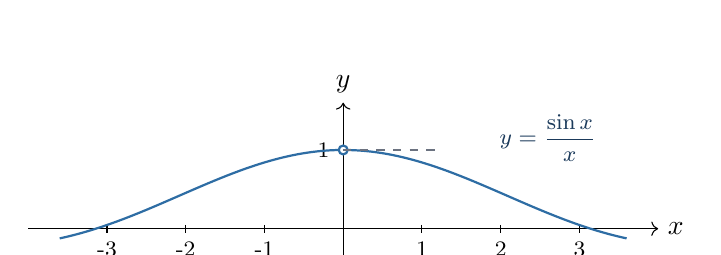
\begin{tikzpicture}[scale=1.0]
\draw[->] (-4,0)--(4,0) node[right]{$x$};
\draw[->] (0,-0.4)--(0,1.6) node[above]{$y$};
\foreach \x in {-3,-2,-1,1,2,3} \draw (\x,0.05)--(\x,-0.05) node[below]{\footnotesize\x};
\draw (0.05,1)--(-0.05,1) node[left]{\footnotesize 1};
% sin(x)/x, x radyan: tikz deg kullanir -> x*57.2958
\draw[grafikMavi,thick,domain=-3.6:3.6,samples=120] plot (\x,{sin(\x r)/(\x)});
\filldraw[white,draw=grafikMavi,thick] (0,1) circle (1.6pt);
\draw[dashed,ortaGri] (0,1)--(1.2,1);
\node[anaMavi] at (2.6,1.15) {\footnotesize $y=\dfrac{\sin x}{x}$};
\end{tikzpicture}
\end{center}

\soru{$\displaystyle \lim_{x \to 0}\frac{\sin 5x}{x}$ limitini hesaplayın.}

\cozum Amacımız ifadeyi $\frac{\sin(\text{şey})}{\text{aynı şey}}$ biçimine
sokmaktır. Pay ve paydayı $5$ ile düzenleriz:
\[
\lim_{x\to0}\frac{\sin 5x}{x} = \lim_{x\to0}\frac{\sin 5x}{5x}\cdot 5
= 5\cdot\underbrace{\lim_{x\to0}\frac{\sin 5x}{5x}}_{=\,1} = 5\cdot 1 = 5 .
\]

\soru{$\displaystyle \lim_{x \to 0}\frac{\sin 3x}{\sin 7x}$ limitini
hesaplayın.}

\cozum Hem payı hem paydayı uygun biçime getiririz:
\[
\frac{\sin 3x}{\sin 7x}
= \frac{\dfrac{\sin 3x}{3x}\cdot 3x}{\dfrac{\sin 7x}{7x}\cdot 7x}
= \frac{\dfrac{\sin 3x}{3x}}{\dfrac{\sin 7x}{7x}}\cdot\frac{3x}{7x}.
\]
$x\to 0$'da iki kesir de $1$'e gider ve $\frac{3x}{7x}=\frac{3}{7}$ kalır:
\[
\lim_{x\to0}\frac{\sin 3x}{\sin 7x} = \frac{1}{1}\cdot\frac{3}{7} = \frac{3}{7}.
\]

\gsub{Sıkıştırma Teoremi (Squeeze Theorem)}

\kural[Squeeze Theorem]{Eğer $a$ civarında $g(x) \le f(x) \le h(x)$ ise ve
$\lm{x}{a}g(x) = \lm{x}{a}h(x) = L$ ise, o zaman $\lm{x}{a}f(x) = L$ olur.
Yani $f$ iki fonksiyon arasında ``sıkışırsa'', onların gittiği yere gitmek
zorundadır.}

\soru{$\displaystyle \lim_{x \to 0}\, x^2 \sin\!\frac{1}{x}$ limitini
hesaplayın.}

\cozum $\sin\frac{1}{x}$ terimi $x=0$'da salınır (limiti yoktur), ama her zaman
$-1 \le \sin\frac{1}{x} \le 1$'dir. Her tarafı $x^2 \ge 0$ ile çarparsak:
\[
-x^2 \le x^2\sin\frac{1}{x} \le x^2 .
\]
Alt ve üst sınırın limitleri: $\lm{x}{0}(-x^2)=0$ ve $\lm{x}{0}x^2=0$. İkisi de
$0$ olduğundan, sıkıştırma teoremiyle:
\[
\lim_{x\to0} x^2\sin\frac{1}{x} = 0 .
\]

% =====================================================================
\gsec{Süreklilik (Continuity)}
% =====================================================================

Sezgisel olarak bir fonksiyon, grafiği ``kalemi kaldırmadan'' çizilebiliyorsa
süreklidir. Matematiksel tanım, limit kavramına dayanır.

\tanim[Süreklilik Tanımı]{$f$ fonksiyonu $x=a$ noktasında \emph{süreklidir}
(continuous), ancak ve ancak şu üç koşul birden sağlanırsa:
\begin{enumerate}\itemsep2pt
\item $f(a)$ \emph{tanımlıdır} (fonksiyonun o noktada değeri var),
\item $\lm{x}{a}f(x)$ \emph{vardır} (limit mevcut),
\item $\lm{x}{a}f(x) = f(a)$ (limit, fonksiyon değerine eşit).
\end{enumerate}}

\gsub{Süreksizlik Türleri (Types of Discontinuity)}

\begin{center}
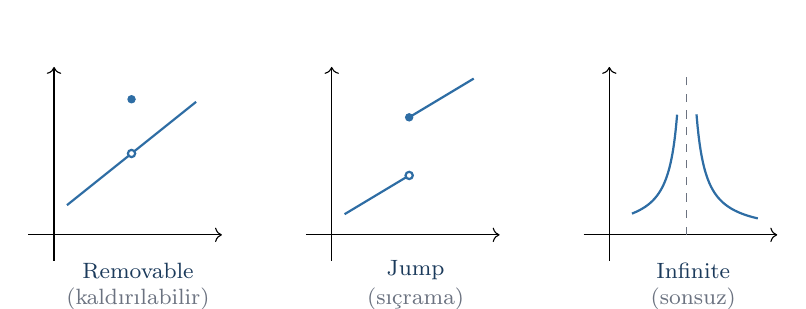
\begin{tikzpicture}[scale=0.82]
% 1) Removable (delik)
\begin{scope}[shift={(0,0)}]
\draw[->] (-0.4,0)--(2.6,0); \draw[->] (0,-0.4)--(0,2.6);
\draw[grafikMavi,thick,domain=0.2:2.2] plot (\x,{0.8*\x+0.3});
\filldraw[white,draw=grafikMavi,thick] (1.2,1.26) circle (1.6pt);
\filldraw[grafikMavi] (1.2,2.1) circle (1.6pt);
\node[anaMavi] at (1.3,-0.55) {\footnotesize Removable};
\node[ortaGri] at (1.3,-1.0) {\footnotesize (kaldırılabilir)};
\end{scope}
% 2) Jump (sıçrama)
\begin{scope}[shift={(4.3,0)}]
\draw[->] (-0.4,0)--(2.6,0); \draw[->] (0,-0.4)--(0,2.6);
\draw[grafikMavi,thick,domain=0.2:1.2] plot (\x,{0.6*\x+0.2});
\filldraw[white,draw=grafikMavi,thick] (1.2,0.92) circle (1.6pt);
\draw[grafikMavi,thick,domain=1.2:2.2] plot (\x,{0.6*\x+1.1});
\filldraw[grafikMavi] (1.2,1.82) circle (1.6pt);
\node[anaMavi] at (1.3,-0.55) {\footnotesize Jump};
\node[ortaGri] at (1.3,-1.0) {\footnotesize (sıçrama)};
\end{scope}
% 3) Infinite (sonsuz)
\begin{scope}[shift={(8.6,0)}]
\draw[->] (-0.4,0)--(2.6,0); \draw[->] (0,-0.4)--(0,2.6);
\draw[dashed,ortaGri] (1.2,0)--(1.2,2.5);
\draw[grafikMavi,thick,domain=0.35:1.05,samples=60] plot (\x,{0.28/(1.2-\x)});
\draw[grafikMavi,thick,domain=1.35:2.3,samples=60] plot (\x,{0.28/(\x-1.2)});
\node[anaMavi] at (1.3,-0.55) {\footnotesize Infinite};
\node[ortaGri] at (1.3,-1.0) {\footnotesize (sonsuz)};
\end{scope}
\end{tikzpicture}
\end{center}

\begin{center}
\begin{tabularx}{\textwidth}{@{}>{\bfseries\color{anaMavi}}l X@{}}
\toprule
\rowcolor{acikMavi}\color{anaMavi}\textbf{Tür} & \color{anaMavi}\textbf{Açıklama}\\
\midrule
Removable & Limit var ama $f(a)$ yok/farklı; ``delik''. Yeniden tanımlayarak giderilebilir.\\
\rowcolor{acikGri} Jump & Soldan ve sağdan limitler farklı; grafikte sıçrama.\\
Infinite & Fonksiyon $\pm\infty$'a gider; dikey asimptot.\\
\bottomrule
\end{tabularx}
\end{center}

\soru{$f(x)=\dfrac{x^2-1}{x-1}$ fonksiyonu $x=1$'de sürekli midir? Değilse
süreksizlik türü nedir ve nasıl giderilir?}

\cozum $f(1)$ tanımsızdır ($\frac{0}{0}$), yani birinci koşul sağlanmaz ---
fonksiyon $x=1$'de \emph{süreksizdir}. Ancak limit vardır:
\[
\lim_{x\to1}\frac{x^2-1}{x-1} = \lim_{x\to1}\frac{(x-1)(x+1)}{x-1}
= \lim_{x\to1}(x+1) = 2 .
\]
Limit var olduğu için bu \emph{removable} (kaldırılabilir) bir süreksizliktir.
$f(1)=2$ olarak tanımlarsak fonksiyon $x=1$'de sürekli hale gelir.

\soru{$f(x)=\begin{cases} x+1, & x \le 2 \\ 3x - 3, & x > 2 \end{cases}$
fonksiyonu $x=2$'de sürekli midir?}

\cozum Üç koşulu kontrol ederiz. \textbf{(1)} $f(2)=2+1=3$ (tanımlı).
\textbf{(2)} Tek taraflı limitler:
\[
\lim_{x\to2^-}f(x)=2+1=3, \qquad \lim_{x\to2^+}f(x)=3\cdot2-3=3 .
\]
İkisi eşit, yani limit var ve $3$'tür. \textbf{(3)} $\lm{x}{2}f(x)=3=f(2)$.
Üç koşul da sağlandığından fonksiyon $x=2$'de \textbf{süreklidir}.

% =====================================================================
\gsec{Sonsuzda Limit ve Asimptotlar}
% =====================================================================

Şimdiye kadar $x$ bir sonlu sayıya yaklaşıyordu. Ayrıca $x$'in
\emph{sonsuza} gitmesi durumunda fonksiyonun davranışını da inceleriz ---
bu, \emph{yatay asimptotları} (horizontal asymptotes) verir.

\gsub{Sonsuzda Limit (Limits at Infinity)}

\kural[Temel Kural]{Herhangi bir pozitif $n$ kuvveti için:
\[
\lim_{x \to \infty}\frac{1}{x^n} = 0, \qquad
\lim_{x \to -\infty}\frac{1}{x^n} = 0 .
\]
Yani $x$ büyüdükçe $\frac{1}{x^n}$ sıfıra gider.}

Rasyonel fonksiyonlarda sonsuzdaki limiti bulmak için, pay ve paydayı
\emph{paydadaki en yüksek dereceli terime} böleriz.

\soru{$\displaystyle \lim_{x \to \infty}\frac{3x^2 + 2x - 1}{5x^2 - x + 4}$
limitini hesaplayın.}

\cozum Pay ve paydayı $x^2$'ye böleriz:
\[
\lim_{x\to\infty}\frac{3 + \frac{2}{x} - \frac{1}{x^2}}
{5 - \frac{1}{x} + \frac{4}{x^2}}
= \frac{3 + 0 - 0}{5 - 0 + 0} = \frac{3}{5}.
\]
$\frac{1}{x}$ ve $\frac{1}{x^2}$ terimleri $x\to\infty$'da sıfıra gider.

\kural[Rasyonel Fonksiyonda Kısayol]{$\dfrac{a_n x^n + \dots}{b_m x^m + \dots}$
için $x\to\pm\infty$ limiti:
\begin{itemize}\itemsep2pt
\item $n < m$ ise limit $0$ (payda daha hızlı büyür),
\item $n = m$ ise limit $\dfrac{a_n}{b_m}$ (baş katsayıların oranı),
\item $n > m$ ise limit $\pm\infty$ (pay daha hızlı büyür).
\end{itemize}}

\gsub{Asimptotlar (Asymptotes)}

\begin{center}
\begin{tabularx}{\textwidth}{@{}>{\bfseries\color{anaMavi}}l X@{}}
\toprule
\rowcolor{acikMavi}\color{anaMavi}\textbf{Asimptot} & \color{anaMavi}\textbf{Nasıl bulunur?}\\
\midrule
Vertical (dikey) & Payda sıfır, pay sıfır değilken: $x=a$ doğrusu. Limit $\pm\infty$.\\
\rowcolor{acikGri} Horizontal (yatay) & $\lm{x}{\pm\infty}f(x)=L$ ise $y=L$ doğrusu.\\
\bottomrule
\end{tabularx}
\end{center}

\soru{$f(x)=\dfrac{2x}{x-1}$ fonksiyonunun dikey ve yatay asimptotlarını
bulun.}

\cozum \textbf{Dikey:} Payda $x-1=0 \Rightarrow x=1$; bu noktada pay
$2\cdot1=2\ne0$. Demek ki $x=1$ dikey asimptottur. \textbf{Yatay:} Pay ve
payda aynı derecede (1), baş katsayı oranı $\frac{2}{1}=2$:
\[
\lim_{x\to\pm\infty}\frac{2x}{x-1} = 2 \;\Rightarrow\; y=2 \text{ yatay asimptot.}
\]

\begin{center}
\begin{tikzpicture}[scale=0.85]
\draw[->] (-3.5,0)--(4.5,0) node[right]{$x$};
\draw[->] (0,-3.5)--(0,4.5) node[above]{$y$};
% asimptotlar
\draw[dashed,kirmizi] (1,-3.3)--(1,4.3) node[above,black]{\footnotesize $x=1$};
\draw[dashed,kirmizi] (-3.3,2)--(4.3,2) node[right,black]{\footnotesize $y=2$};
% f(x)=2x/(x-1), iki kol
\draw[grafikMavi,thick,domain=-3.3:0.6,samples=80] plot (\x,{2*\x/(\x-1)});
\draw[grafikMavi,thick,domain=1.45:4.3,samples=80] plot (\x,{2*\x/(\x-1)});
\node[anaMavi] at (3.3,3.4) {\footnotesize $y=\dfrac{2x}{x-1}$};
\end{tikzpicture}
\end{center}

\bilgi{\textbf{Kısım 1 özeti:} Limit, $x\to a$ iken $f(x)$'in yaklaştığı
değerdir --- $f(a)$ ile aynı olmak zorunda değildir. Hesaplarken önce yerine
koy; $\frac{0}{0}$ çıkarsa çarpanlara ayır / eşlenikle çarp. Süreklilik,
limitin fonksiyon değerine eşit olmasıdır. Sonsuzda limit yatay asimptotu,
paydanın sıfırı dikey asimptotu verir. Şimdi bu temeli kullanarak
\emph{türeve} geçebiliriz --- çünkü türev, özünde bir limittir.}

% #####################################################################
\gpart{2}{Türev (Derivative)}
% #####################################################################

% =====================================================================
\gsec{Türevin Tanımı ve Teğet Doğru}
% =====================================================================

Türev (derivative), bir fonksiyonun \emph{anlık değişim oranını} ölçer:
``$x$ birazcık değişince $f(x)$ ne kadar değişir?'' Geometrik olarak türev,
bir noktadaki \emph{teğet doğrunun eğimidir} (slope of the tangent line).

\gsub{Kesen Doğrudan Teğet Doğruya}

Bir eğri üzerindeki iki noktadan geçen doğruya \emph{kesen} (secant) denir;
eğimi ortalama değişim oranıdır. İki nokta birbirine yaklaştıkça kesen,
\emph{teğet} (tangent) doğruya dönüşür --- işte türev bu limittir.

\begin{center}
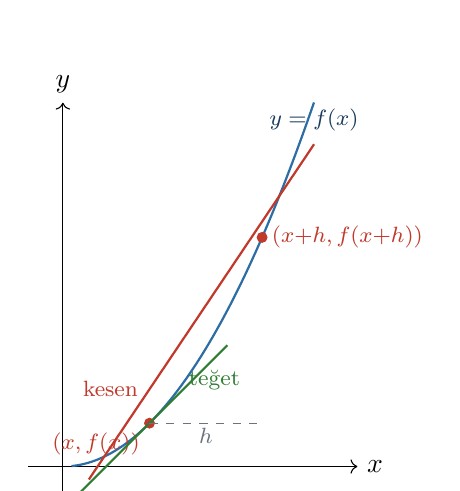
\begin{tikzpicture}[scale=1.1]
\draw[->] (-0.4,0)--(3.4,0) node[right]{$x$};
\draw[->] (0,-0.4)--(0,4.2) node[above]{$y$};
\draw[grafikMavi,thick,domain=0.1:2.9,samples=100] plot (\x,{0.5*\x*\x});
% nokta a=1 ve a+h=2.3
\filldraw[kirmizi] (1,0.5) circle (1.6pt) node[below left]{\footnotesize $(x,f(x))$};
\filldraw[kirmizi] (2.3,2.645) circle (1.6pt) node[right]{\footnotesize $(x{+}h,f(x{+}h))$};
% kesen dogru
\draw[kirmizi,thick] (0.3,-0.15)--(2.9,3.72);
\node[kirmizi] at (0.55,0.9) {\footnotesize kesen};
% tegetin egimi noktada
\draw[yesil,thick] (0.2,-0.3)--(1.9,1.4);
\node[yesil] at (1.75,1.0) {\footnotesize teğet};
% h araligi
\draw[dashed,ortaGri] (1,0.5)--(2.3,0.5);
\node[ortaGri] at (1.65,0.35) {\footnotesize $h$};
\node[anaMavi] at (2.9,4.0) {\footnotesize $y=f(x)$};
\end{tikzpicture}
\end{center}

\tanim[Türevin Limit Tanımı]{$f$ fonksiyonunun $x$ noktasındaki türevi:
\[
f'(x) = \lim_{h \to 0}\frac{f(x+h) - f(x)}{h},
\]
bu limit var olduğu takdirde. Gösterimler: $f'(x)$, $\dfrac{dy}{dx}$,
$\dfrac{df}{dx}$, $Df$. Kesirdeki $\frac{f(x+h)-f(x)}{h}$ ifadesine
\emph{fark bölümü} (difference quotient) denir.}

\gsub{Tanımdan Türev Alma (First Principles)}

\soru{$f(x)=x^2$ fonksiyonunun türevini \emph{limit tanımını} kullanarak
bulun.}

\cozum Fark bölümünü kurup limitini alırız:
\[
f'(x) = \lim_{h\to0}\frac{(x+h)^2 - x^2}{h}
= \lim_{h\to0}\frac{x^2 + 2xh + h^2 - x^2}{h}
= \lim_{h\to0}\frac{2xh + h^2}{h}.
\]
Pay ve paydadan $h$ sadeleşir:
\[
= \lim_{h\to0}(2x + h) = 2x .
\]
Yani $\dfrac{d}{dx}x^2 = 2x$. Örneğin $x=3$'te eğim $f'(3)=6$'dır.

\soru{$f(x)=\dfrac{1}{x}$ fonksiyonunun türevini limit tanımıyla bulun.}

\cozum
\[
f'(x)=\lim_{h\to0}\frac{\frac{1}{x+h}-\frac{1}{x}}{h}
=\lim_{h\to0}\frac{\frac{x-(x+h)}{x(x+h)}}{h}
=\lim_{h\to0}\frac{-h}{h\,x(x+h)}
=\lim_{h\to0}\frac{-1}{x(x+h)} = -\frac{1}{x^2}.
\]

\gsub{Teğet Doğrunun Denklemi}

Bir noktadaki türev eğimi verdiğine göre, o noktadaki teğet doğrunun denklemini
nokta-eğim formuyla yazabiliriz: $y - f(a) = f'(a)\,(x - a)$.

\soru{$f(x)=x^2$ eğrisine $x=3$ noktasındaki teğet doğrunun denklemini bulun.}

\cozum Nokta: $f(3)=9$, yani $(3,9)$. Eğim: $f'(x)=2x \Rightarrow f'(3)=6$.
Teğet doğru:
\[
y - 9 = 6(x - 3) \;\Longrightarrow\; y = 6x - 9 .
\]

% =====================================================================
\gsec{Türev Kuralları}
% =====================================================================

Her türevi limit tanımıyla almak zahmetlidir. Neyse ki türev almayı
mekanikleştiren kurallar vardır. Bu bölüm, türev hesaplamanın araç kutusudur.

\gsub{Temel Kurallar}

\begin{center}
\begin{tabularx}{\textwidth}{@{}>{\bfseries\color{anaMavi}}l >{$}l<{$} X@{}}
\toprule
\rowcolor{acikMavi}\color{anaMavi}\textbf{Kural} & \color{anaMavi}\textbf{Formül} & \color{anaMavi}\textbf{Örnek}\\
\midrule
Sabit & \dfrac{d}{dx}c = 0 & $(7)'=0$\\
\rowcolor{acikGri} Kuvvet (power) & \dfrac{d}{dx}x^n = n x^{n-1} & $(x^5)'=5x^4$\\
Sabit katı & (c\,f)' = c\,f' & $(3x^2)'=6x$\\
Toplam/fark & (f\pm g)' = f' \pm g' & $(x^2+x)'=2x+1$\\
\bottomrule
\end{tabularx}
\end{center}

\soru{$f(x)=4x^3 - 2x^2 + 7x - 5$ fonksiyonunun türevini bulun.}

\cozum Her terime kuvvet kuralını uygularız:
\[
f'(x) = 4\cdot3x^2 - 2\cdot2x + 7\cdot1 - 0 = 12x^2 - 4x + 7 .
\]

\soru{$f(x)=\sqrt{x} + \dfrac{1}{x^2}$ fonksiyonunun türevini bulun.}

\cozum Önce kuvvet biçiminde yazarız: $\sqrt{x}=x^{1/2}$, $\frac{1}{x^2}=x^{-2}$.
\[
f'(x) = \tfrac{1}{2}x^{-1/2} + (-2)x^{-3}
= \frac{1}{2\sqrt{x}} - \frac{2}{x^3}.
\]

\gsub{Çarpım ve Bölüm Kuralı (Product \& Quotient Rule)}

\kural[Product Rule]{$(f\cdot g)' = f'\,g + f\,g'$. \\[2pt]
\textbf{Quotient Rule:} $\left(\dfrac{f}{g}\right)' = \dfrac{f'\,g - f\,g'}{g^2}$.}

\soru{$f(x)=(x^2+1)(x^3-2x)$ fonksiyonunun türevini çarpım kuralıyla bulun.}

\cozum $f'=(x^2+1)'(x^3-2x)+(x^2+1)(x^3-2x)'$. Parçalar:
$(x^2+1)'=2x$ ve $(x^3-2x)'=3x^2-2$.
\[
f'(x) = 2x(x^3-2x) + (x^2+1)(3x^2-2)
= 2x^4 - 4x^2 + 3x^4 + x^2 - 2 = 5x^4 - 3x^2 - 2 .
\]

\soru{$f(x)=\dfrac{x}{x^2+1}$ fonksiyonunun türevini bölüm kuralıyla bulun.}

\cozum $f=\frac{u}{v}$, $u=x$, $v=x^2+1$; $u'=1$, $v'=2x$.
\[
f'(x) = \frac{u'v - uv'}{v^2} = \frac{1\cdot(x^2+1) - x\cdot 2x}{(x^2+1)^2}
= \frac{x^2+1-2x^2}{(x^2+1)^2} = \frac{1-x^2}{(x^2+1)^2}.
\]

\gsub{Zincir Kuralı (Chain Rule)}

Zincir kuralı, \emph{bileşke fonksiyonların} (function of a function) türevi
içindir --- ve pratikte en çok kullanılan kuraldır.

\kural[Chain Rule]{$\dfrac{d}{dx}f(g(x)) = f'(g(x))\cdot g'(x)$. \\[2pt]
Sözle: ``dıştakinin türevi (içteki aynen) çarpı içtekinin türevi''.}

\soru{$f(x)=(3x^2+1)^5$ fonksiyonunun türevini bulun.}

\cozum Dış fonksiyon $(\cdot)^5$, iç fonksiyon $3x^2+1$. Zincir kuralı:
\[
f'(x) = 5(3x^2+1)^4 \cdot \underbrace{(6x)}_{\text{için türevi}}
= 30x\,(3x^2+1)^4 .
\]

\soru{$f(x)=\sqrt{x^2 + 9}$ fonksiyonunun türevini bulun.}

\cozum $f(x)=(x^2+9)^{1/2}$. Dış: $(\cdot)^{1/2}$, iç: $x^2+9$.
\[
f'(x) = \tfrac{1}{2}(x^2+9)^{-1/2}\cdot 2x = \frac{x}{\sqrt{x^2+9}}.
\]

% =====================================================================
\gsec{Trigonometrik, Üstel ve Logaritmik Türevler}
% =====================================================================

\gsub{Türev Tablosu}

\begin{center}
\begin{tabularx}{\textwidth}{@{}>{$}l<{$} >{$}l<{$} X@{}}
\toprule
\rowcolor{acikMavi}\color{anaMavi}\textbf{f(x)} & \color{anaMavi}\textbf{f'(x)} & \\
\midrule
\sin x & \cos x & \\
\rowcolor{acikGri} \cos x & -\sin x & (işaret değişir)\\
\tan x & \sec^2 x & \\
\rowcolor{acikGri} e^x & e^x & (kendi türevine eşit)\\
a^x & a^x \ln a & \\
\rowcolor{acikGri} \ln x & \dfrac{1}{x} & $(x>0)$\\
\log_a x & \dfrac{1}{x\ln a} & \\
\bottomrule
\end{tabularx}
\end{center}

\soru{$f(x)=e^{2x}\sin x$ fonksiyonunun türevini bulun.}

\cozum Çarpım kuralı + zincir kuralı ($e^{2x}$ için). $(e^{2x})'=2e^{2x}$.
\[
f'(x) = (e^{2x})'\sin x + e^{2x}(\sin x)'
= 2e^{2x}\sin x + e^{2x}\cos x = e^{2x}(2\sin x + \cos x).
\]

\soru{$f(x)=\ln(x^2 + 1)$ fonksiyonunun türevini bulun.}

\cozum Zincir kuralı: $(\ln u)'=\frac{u'}{u}$, $u=x^2+1$, $u'=2x$.
\[
f'(x) = \frac{2x}{x^2+1}.
\]

\gsub{Kapalı Türev (Implicit Differentiation)}

$y$ açıkça $x$ cinsinden yazılamıyorsa (örneğin $x^2+y^2=25$), denklemin her
iki tarafının türevini alırız; $y$ terimlerinin türevinde zincir kuralıyla
$\frac{dy}{dx}$ çarpanı ekleriz.

\soru{$x^2 + y^2 = 25$ çemberinde $\dfrac{dy}{dx}$'i bulun.}

\cozum Her iki tarafın $x$'e göre türevini alırız ($y$, $x$'in fonksiyonudur):
\[
2x + 2y\frac{dy}{dx} = 0 \;\Longrightarrow\;
\frac{dy}{dx} = -\frac{x}{y}.
\]
Örneğin $(3,4)$ noktasında teğet eğimi $-\frac{3}{4}$'tür.

\gsub{İkinci Türev (Second Derivative)}

Türevin türevine \emph{ikinci türev} denir: $f''(x)=\frac{d}{dx}f'(x)$.
Fiziksel anlamı: konum $\to$ hız (1. türev) $\to$ ivme (2. türev). Grafikte
ise \emph{konkavlığı} (bükeylik) belirler.

\soru{$f(x)=x^4 - 3x^2$ için $f''(x)$'i bulun.}

\cozum Önce birinci türev: $f'(x)=4x^3-6x$. Sonra tekrar türev:
\[
f''(x) = 12x^2 - 6 .
\]

% =====================================================================
\gsec{Türevin Uygulamaları}
% =====================================================================

Türev, bir fonksiyonun grafiğini analiz etmenin ve gerçek dünya optimizasyon
problemlerini çözmenin en güçlü aracıdır.

\gsub{Artan/Azalan ve Ekstremum}

\kural[Birinci Türev Testi]{$f'(x) > 0$ olan aralıkta $f$ \emph{artandır}
(increasing); $f'(x) < 0$ olan aralıkta \emph{azalandır} (decreasing).
$f'(x)=0$ (veya tanımsız) olan noktalara \emph{kritik nokta} (critical point)
denir; yerel maksimum/minimum buralarda olur.
\begin{itemize}\itemsep2pt
\item $f'$ kritik noktada $+$'dan $-$'ye geçiyorsa: yerel \textbf{maksimum}.
\item $f'$ kritik noktada $-$'den $+$'ya geçiyorsa: yerel \textbf{minimum}.
\end{itemize}}

\soru{$f(x)=x^3 - 3x^2 + 4$ fonksiyonunun yerel maksimum ve minimumlarını
bulun.}

\cozum Kritik noktalar için $f'(x)=0$:
\[
f'(x) = 3x^2 - 6x = 3x(x-2) = 0 \;\Rightarrow\; x=0 \text{ veya } x=2 .
\]
İşaret incelemesi: $f'$, $x<0$ için $+$, $0<x<2$ için $-$, $x>2$ için $+$.
Demek ki $x=0$'da $+\to-$: \textbf{yerel maksimum} $f(0)=4$; $x=2$'de $-\to+$:
\textbf{yerel minimum} $f(2)=8-12+4=0$.

\begin{center}
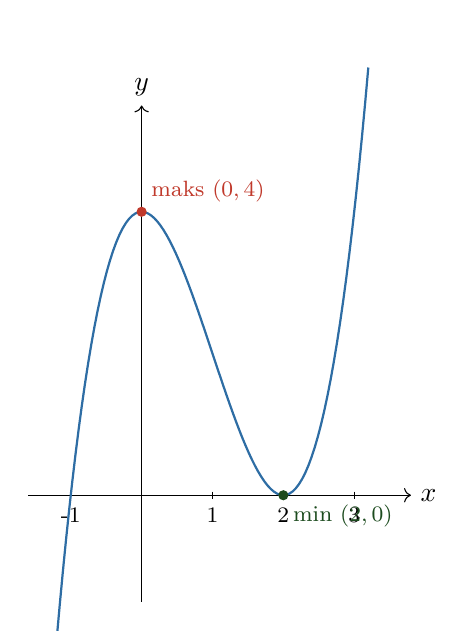
\begin{tikzpicture}[scale=0.9]
\draw[->] (-1.6,0)--(3.8,0) node[right]{$x$};
\draw[->] (0,-1.5)--(0,5.5) node[above]{$y$};
\foreach \x in {-1,1,2,3} \draw (\x,0.05)--(\x,-0.05) node[below]{\footnotesize\x};
\draw[grafikMavi,thick,domain=-1.2:3.2,samples=100] plot (\x,{\x*\x*\x-3*\x*\x+4});
\filldraw[kirmizi] (0,4) circle (1.8pt) node[above right]{\footnotesize maks $(0,4)$};
\filldraw[yesil!60!black] (2,0) circle (1.8pt) node[below right]{\footnotesize min $(2,0)$};
\end{tikzpicture}
\end{center}

\gsub{Konkavlık ve Büküm Noktası (Concavity \& Inflection)}

\kural[İkinci Türev Testi]{$f''(x)>0$ ise grafik \emph{konkav yukarı}
(çanak $\smile$); $f''(x)<0$ ise \emph{konkav aşağı} (kubbe $\frown$).
Konkavlığın değiştiği noktaya \emph{büküm noktası} (inflection point) denir;
orada $f''(x)=0$'dır. Ayrıca bir kritik noktada $f''>0$ ise yerel minimum,
$f''<0$ ise yerel maksimum vardır.}

\gsub{Optimizasyon Problemleri}

Türevin en pratik uygulaması: bir büyüklüğü maksimize veya minimize etmek.

\soru{Çevresi 40 m olan dikdörtgen bir bahçenin \emph{en büyük alanı} ne olur?}

\cozum Kenarlar $x$ ve $y$ olsun. Çevre kısıtı: $2x+2y=40 \Rightarrow y=20-x$.
Alan fonksiyonu:
\[
A(x) = x\,y = x(20-x) = 20x - x^2 .
\]
Maksimum için türevi sıfırlarız: $A'(x)=20-2x=0 \Rightarrow x=10$. İkinci türev
$A''=-2<0$ olduğundan bu bir maksimumdur. $y=20-10=10$. Yani kare
($10\times10$) en büyük alanı verir: $A=100\ \text{m}^2$.

\soru{Bir top yukarı atılıyor; yüksekliği $h(t)=-5t^2 + 20t + 1$ (metre).
Topun ulaştığı en yüksek noktayı bulun.}

\cozum Hız $h'(t)=-10t+20$. En yüksek noktada hız sıfırdır:
$-10t+20=0 \Rightarrow t=2$ s. Bu andaki yükseklik:
\[
h(2) = -5(4) + 20(2) + 1 = -20 + 40 + 1 = 21 \text{ m}.
\]

\gsub{L'Hôpital Kuralı}

Belirsiz limitler ($\frac{0}{0}$ veya $\frac{\infty}{\infty}$) türevle çok
kolay çözülür.

\kural[L'Hôpital's Rule]{$\lm{x}{a}\dfrac{f(x)}{g(x)}$ limiti $\frac{0}{0}$
veya $\frac{\infty}{\infty}$ belirsizliğindeyse:
\[
\lim_{x\to a}\frac{f(x)}{g(x)} = \lim_{x\to a}\frac{f'(x)}{g'(x)},
\]
sağdaki limit var olduğu sürece. (Pay ve paydanın \emph{ayrı ayrı} türevi
alınır --- bölüm kuralı değil!)}

\soru{$\displaystyle \lim_{x \to 0}\frac{\sin x}{x}$ limitini L'Hôpital ile
hesaplayın.}

\cozum $\frac{0}{0}$ belirsizliği. Pay ve paydanın türevini alırız:
$(\sin x)'=\cos x$, $(x)'=1$.
\[
\lim_{x\to0}\frac{\sin x}{x} = \lim_{x\to0}\frac{\cos x}{1} = \cos 0 = 1 .
\]
(Bölüm 3'te bunu geometrik olarak da bulmuştuk --- iki yöntem aynı sonucu verir.)

\soru{$\displaystyle \lim_{x \to \infty}\frac{e^x}{x^2}$ limitini hesaplayın.}

\cozum $\frac{\infty}{\infty}$ belirsizliği. L'Hôpital'i \emph{iki kez}
uygularız:
\[
\lim_{x\to\infty}\frac{e^x}{x^2}
= \lim_{x\to\infty}\frac{e^x}{2x}
= \lim_{x\to\infty}\frac{e^x}{2} = \infty .
\]
Bu, üstel fonksiyonun polinomdan çok daha hızlı büyüdüğünü gösterir.

\bilgi{\textbf{Kısım 2 özeti:} Türev, teğetin eğimi ve anlık değişim oranıdır;
tanımı bir limittir ama pratikte kurallarla (power, product, quotient, chain)
hesaplanır. $f'$ artan/azalanı ve ekstremumları, $f''$ konkavlığı verir.
Optimizasyon: kısıtı kullanıp tek değişkenli bir fonksiyon kur, türevini
sıfırla. L'Hôpital belirsiz limitleri türevle çözer. Şimdi türevin tersi olan
\emph{integrale} geçiyoruz.}

% #####################################################################
\gpart{3}{İntegral}
% #####################################################################

% =====================================================================
\gsec{Belirsiz İntegral (Antiderivative)}
% =====================================================================

İntegral, türevin \emph{ters işlemidir}. Türev ``$f$'nin değişim oranı nedir?''
diye sorarken, integral ``türevi $f$ olan fonksiyon nedir?'' diye sorar.
Bu fonksiyona \emph{ters türev} (antiderivative) veya \emph{belirsiz integral}
denir.

\tanim[Belirsiz İntegral]{$F'(x) = f(x)$ ise, $F$ fonksiyonu $f$'nin bir ters
türevidir ve şöyle yazılır:
\[
\int f(x)\,dx = F(x) + C .
\]
Buradaki $C$ \emph{integral sabitidir} (constant of integration): herhangi bir
sabitin türevi sıfır olduğundan, ters türev bir sabit farkıyla belirsizdir ---
bu yüzden ``belirsiz'' integral.}

\uyari{$+C$'yi \textbf{asla unutma!} $\frac{d}{dx}(x^2)=2x$ ama
$\frac{d}{dx}(x^2+7)=2x$ de doğrudur. Yani $\int 2x\,dx = x^2 + C$; sabit
kaybolduğundan geri getirmek zorundayız. Belirli integralde (birazdan) $C$
sadeleşir, ama belirsiz integralde şarttır.}

\gsub{Temel İntegral Kuralları}

Her türev kuralı, tersten okununca bir integral kuralı verir.

\begin{center}
\begin{tabularx}{\textwidth}{@{}>{$}l<{$} >{$}l<{$} X@{}}
\toprule
\rowcolor{acikMavi}\color{anaMavi}\int f(x)\,dx & \color{anaMavi}\text{Sonuç} & \\
\midrule
\int x^n\,dx & \dfrac{x^{n+1}}{n+1} + C & $(n\ne -1)$\\
\rowcolor{acikGri} \int \dfrac{1}{x}\,dx & \ln|x| + C & ($n=-1$ durumu)\\
\int e^x\,dx & e^x + C & \\
\rowcolor{acikGri} \int \cos x\,dx & \sin x + C & \\
\int \sin x\,dx & -\cos x + C & (işaret!)\\
\rowcolor{acikGri} \int \sec^2 x\,dx & \tan x + C & \\
\bottomrule
\end{tabularx}
\end{center}

\kural[Power Rule for Integrals]{Üssü \emph{bir artır, ona böl}:
$\displaystyle\int x^n\,dx = \frac{x^{n+1}}{n+1} + C$. (Türevdeki ``üssü indir,
bir azalt'' kuralının tam tersi.)}

\soru{$\displaystyle \int (3x^2 - 4x + 5)\,dx$ integralini hesaplayın.}

\cozum Her terimi ayrı ayrı integre ederiz:
\[
\int 3x^2\,dx - \int 4x\,dx + \int 5\,dx
= 3\cdot\frac{x^3}{3} - 4\cdot\frac{x^2}{2} + 5x + C
= x^3 - 2x^2 + 5x + C .
\]
\textbf{Kontrol:} Sonucun türevini alırsak $3x^2-4x+5$ --- başladığımız ifade.
Türev alarak integralini her zaman doğrulayabilirsin.

\soru{$\displaystyle \int \left(\sqrt{x} + \frac{1}{x^2}\right)dx$ integralini
hesaplayın.}

\cozum Kuvvet biçiminde yazarız: $\sqrt{x}=x^{1/2}$, $\frac{1}{x^2}=x^{-2}$.
\[
\int x^{1/2}\,dx + \int x^{-2}\,dx
= \frac{x^{3/2}}{3/2} + \frac{x^{-1}}{-1} + C
= \frac{2}{3}x^{3/2} - \frac{1}{x} + C .
\]

% =====================================================================
\gsec{İntegral Teknikleri}
% =====================================================================

Temel kurallar yetmediğinde, integrali çözülebilir bir biçime dönüştüren
teknikler kullanırız. En önemlileri: yerine koyma ve kısmi integral.

\gsub{Yerine Koyma (u-Substitution)}

Zincir kuralının tersidir. İntegralin içinde bir fonksiyon ve
(katsayı farkıyla) onun türevi varsa, o fonksiyonu $u$ olarak adlandırıp
integrali basitleştiririz.

\kural[u-Substitution]{$\displaystyle\int f(g(x))\,g'(x)\,dx$ için $u=g(x)$,
$du=g'(x)\,dx$ dönüşümü yapılır; integral $\int f(u)\,du$ biçimine iner.}

\soru{$\displaystyle \int 2x\,(x^2+1)^3\,dx$ integralini hesaplayın.}

\cozum $u=x^2+1$ seçelim. O zaman $du=2x\,dx$ --- ki bu tam olarak integralde
mevcut! Dönüştürürüz:
\[
\int (x^2+1)^3\,(2x\,dx) = \int u^3\,du = \frac{u^4}{4} + C
= \frac{(x^2+1)^4}{4} + C .
\]

\soru{$\displaystyle \int \frac{x}{x^2+1}\,dx$ integralini hesaplayın.}

\cozum $u=x^2+1$, $du=2x\,dx \Rightarrow x\,dx=\frac{1}{2}du$.
\[
\int\frac{x\,dx}{x^2+1} = \int\frac{\frac{1}{2}du}{u}
= \frac{1}{2}\int\frac{du}{u} = \frac{1}{2}\ln|u| + C
= \frac{1}{2}\ln(x^2+1) + C .
\]

\gsub{Kısmi İntegral (Integration by Parts)}

Çarpım kuralının tersidir. İki fonksiyonun \emph{çarpımını} integre ederken
kullanılır (özellikle $x e^x$, $x\sin x$, $\ln x$ gibi).

\kural[Integration by Parts]{$\displaystyle\int u\,dv = uv - \int v\,du$. \\[2pt]
$u$ seçimi için \textbf{LIATE} sırası yardımcı olur: \textbf{L}ogaritmik,
\textbf{I}nvers trig, \textbf{A}lgebraik, \textbf{T}rigonometrik,
\textbf{E}xponansiyel --- listede önce gelen $u$ olur.}

\soru{$\displaystyle \int x\,e^x\,dx$ integralini hesaplayın.}

\cozum LIATE: Algebraik ($x$), Exponansiyel'den ($e^x$) önce gelir, yani $u=x$.
Seçimler: $u=x \Rightarrow du=dx$; \ $dv=e^x dx \Rightarrow v=e^x$.
\[
\int x e^x\,dx = uv - \int v\,du = x e^x - \int e^x\,dx = x e^x - e^x + C
= e^x(x-1) + C .
\]

\soru{$\displaystyle \int \ln x\,dx$ integralini hesaplayın.}

\cozum Görünürde çarpım yok ama $\ln x = \ln x \cdot 1$ diye düşünürüz.
$u=\ln x \Rightarrow du=\frac{1}{x}dx$; \ $dv=dx \Rightarrow v=x$.
\[
\int \ln x\,dx = x\ln x - \int x\cdot\frac{1}{x}\,dx = x\ln x - \int 1\,dx
= x\ln x - x + C .
\]

\gsub{Kısmi Kesirler (Partial Fractions)}

Rasyonel bir ifadeyi (payda çarpanlara ayrılabiliyorsa) daha basit kesirlerin
toplamına ayırıp integre ederiz.

\soru{$\displaystyle \int \frac{1}{x^2 - 1}\,dx$ integralini hesaplayın.}

\cozum Payda $x^2-1=(x-1)(x+1)$. Kısmi kesirlere ayırırız:
\[
\frac{1}{(x-1)(x+1)} = \frac{A}{x-1} + \frac{B}{x+1}.
\]
$1 = A(x+1)+B(x-1)$. $x=1$: $1=2A \Rightarrow A=\frac{1}{2}$. $x=-1$:
$1=-2B \Rightarrow B=-\frac{1}{2}$. İntegral:
\[
\int\!\left(\frac{1/2}{x-1} - \frac{1/2}{x+1}\right)dx
= \frac{1}{2}\ln|x-1| - \frac{1}{2}\ln|x+1| + C
= \frac{1}{2}\ln\left|\frac{x-1}{x+1}\right| + C .
\]

% =====================================================================
\gsec{Belirli İntegral ve Temel Teorem}
% =====================================================================

Belirsiz integral bir \emph{fonksiyon} verir; \emph{belirli integral}
(definite integral) ise bir \emph{sayı} verir --- geometrik olarak bir eğrinin
altındaki \textbf{alanı}.

\gsub{Riemann Toplamı: Alanı Yaklaşık Hesaplama}

Bir eğri altındaki alanı, onu ince dikdörtgenlere bölüp toplayarak yaklaşık
buluruz. Dikdörtgen sayısı arttıkça (genişlik $\to 0$) yaklaşım gerçek alana
yakınsar --- işte belirli integral bu limittir.

\begin{center}
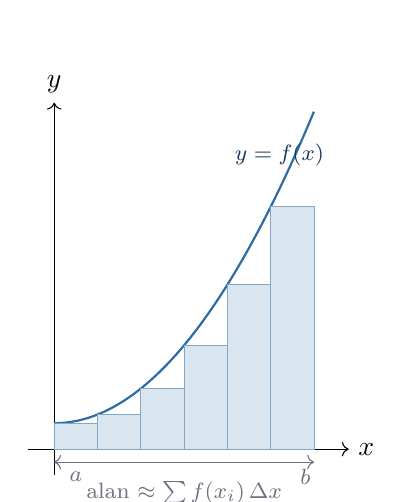
\begin{tikzpicture}[scale=1.1]
\draw[->] (-0.3,0)--(3.4,0) node[right]{$x$};
\draw[->] (0,-0.3)--(0,4) node[above]{$y$};
% egri f(x)=0.4x^2+0.3
\draw[grafikMavi,thick,domain=0:3,samples=100] plot (\x,{0.4*\x*\x+0.3});
% dikdortgenler (sol uc)
\foreach \i in {0,1,2,3,4,5} {
  \pgfmathsetmacro{\xa}{0.5*\i}
  \pgfmathsetmacro{\hh}{0.4*\xa*\xa+0.3}
  \draw[fill=grafikMavi!18,draw=grafikMavi!60] (\xa,0) rectangle (\xa+0.5,\hh);
}
\node[anaMavi] at (2.6,3.4) {\footnotesize $y=f(x)$};
\node[ortaGri] at (1.5,-0.5) {\footnotesize alan $\approx \sum f(x_i)\,\Delta x$};
\draw[<->,ortaGri] (0,-0.15)--(3,-0.15);
\node[ortaGri] at (0.25,-0.32) {\footnotesize $a$};
\node[ortaGri] at (2.9,-0.32) {\footnotesize $b$};
\end{tikzpicture}
\end{center}

\tanim[Belirli İntegral]{$[a,b]$ aralığında $f$'nin belirli integrali, Riemann
toplamının limitidir:
\[
\int_a^b f(x)\,dx = \lim_{n\to\infty}\sum_{i=1}^{n} f(x_i)\,\Delta x,
\qquad \Delta x = \frac{b-a}{n}.
\]
$a$ ve $b$'ye \emph{integral sınırları} (limits of integration) denir.}

\gsub{Kalkülüsün Temel Teoremi (Fundamental Theorem of Calculus)}

Bu teorem, kalkülüsün kalbidir: türev ve integralin \emph{ters işlemler}
olduğunu söyler ve belirli integrali Riemann toplamı olmadan, ters türevle
hesaplamamızı sağlar.

\kural[FTC --- Part 2]{$F$, $f$'nin herhangi bir ters türeviyse ($F'=f$):
\[
\int_a^b f(x)\,dx = F(b) - F(a) \;\equiv\; \Big[F(x)\Big]_a^b .
\]
Yani: ters türevi bul, üst sınırda değerinden alt sınırdaki değerini çıkar.
($C$ sabiti çıkarımda sadeleşir, bu yüzden belirli integralde yazılmaz.)}

\soru{$\displaystyle \int_1^3 x^2\,dx$ belirli integralini hesaplayın.}

\cozum Ters türev $\frac{x^3}{3}$. FTC uygularız:
\[
\int_1^3 x^2\,dx = \left[\frac{x^3}{3}\right]_1^3
= \frac{3^3}{3} - \frac{1^3}{3} = \frac{27}{3} - \frac{1}{3}
= 9 - \frac{1}{3} = \frac{26}{3}.
\]

\soru{$\displaystyle \int_0^{\pi} \sin x\,dx$ belirli integralini hesaplayın.}

\cozum Ters türev $-\cos x$.
\[
\int_0^\pi \sin x\,dx = \Big[-\cos x\Big]_0^\pi
= (-\cos\pi) - (-\cos 0) = -(-1) - (-1) = 1 + 1 = 2 .
\]

\gsub{Belirli İntegralde Yerine Koyma}

Yerine koyma yaparken \emph{sınırları da} yeni değişkene çevirmek pratiktir.

\soru{$\displaystyle \int_0^2 2x\,(x^2+1)^3\,dx$ integralini hesaplayın.}

\cozum $u=x^2+1$, $du=2x\,dx$. Sınırları çeviririz: $x=0 \Rightarrow u=1$;
$x=2 \Rightarrow u=5$.
\[
\int_0^2 2x(x^2+1)^3\,dx = \int_1^5 u^3\,du
= \left[\frac{u^4}{4}\right]_1^5 = \frac{625}{4} - \frac{1}{4}
= \frac{624}{4} = 156 .
\]

% =====================================================================
\gsec{İntegralin Uygulamaları: Alan ve Hacim}
% =====================================================================

\gsub{İki Eğri Arasındaki Alan}

İki eğri arasındaki alan, ``üstteki eksi alttaki'' fonksiyonun integralidir.

\kural[Area Between Curves]{$[a,b]$'de $f(x)\ge g(x)$ ise, aralarındaki alan:
\[
A = \int_a^b \big[f(x) - g(x)\big]\,dx .
\]}

\soru{$y=x$ doğrusu ile $y=x^2$ parabolü arasındaki alanı bulun.}

\cozum Önce kesişim noktaları: $x=x^2 \Rightarrow x^2-x=0 \Rightarrow x=0,1$.
$[0,1]$'de $x \ge x^2$ (doğru üstte). Alan:
\[
A = \int_0^1 (x - x^2)\,dx
= \left[\frac{x^2}{2} - \frac{x^3}{3}\right]_0^1
= \frac{1}{2} - \frac{1}{3} = \frac{1}{6}.
\]

\begin{center}
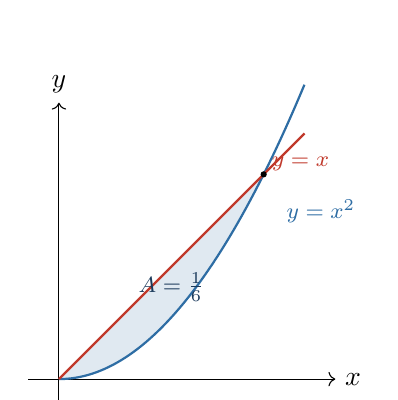
\begin{tikzpicture}[scale=2.6]
\draw[->] (-0.15,0)--(1.35,0) node[right]{$x$};
\draw[->] (0,-0.15)--(0,1.35) node[above]{$y$};
% alan taramasi
\begin{scope}
\clip (0,0) -- plot[domain=0:1,samples=50] (\x,\x) -- plot[domain=1:0,samples=50] (\x,{\x*\x}) -- cycle;
\fill[grafikMavi!15] (0,0) rectangle (1.1,1.1);
\end{scope}
\draw[grafikMavi,thick,domain=0:1.2,samples=60] plot (\x,{\x*\x});
\draw[kirmizi,thick,domain=0:1.2] plot (\x,\x);
\filldraw[black] (1,1) circle (0.35pt);
\node[kirmizi] at (1.18,1.05) {\footnotesize $y=x$};
\node[grafikMavi] at (1.28,0.82) {\footnotesize $y=x^2$};
\node[anaMavi] at (0.55,0.45) {\footnotesize $A=\frac{1}{6}$};
\end{tikzpicture}
\end{center}

\gsub{Dönel Hacim (Volume of Revolution)}

Bir bölgeyi bir eksen etrafında döndürünce oluşan katının hacmini,
\emph{disk yöntemiyle} buluruz: her dilim yarıçapı $f(x)$ olan bir dairedir,
alanı $\pi f(x)^2$.

\kural[Disk Method]{$y=f(x)$ eğrisinin $[a,b]$'deki bölgesini $x$ ekseni
etrafında döndürünce oluşan hacim:
\[
V = \pi\int_a^b \big[f(x)\big]^2\,dx .
\]}

\soru{$y=\sqrt{x}$ eğrisinin $[0,4]$ aralığındaki bölgesini $x$ ekseni
etrafında döndürünce oluşan hacmi bulun.}

\cozum $f(x)=\sqrt{x} \Rightarrow [f(x)]^2 = x$. Disk yöntemi:
\[
V = \pi\int_0^4 x\,dx = \pi\left[\frac{x^2}{2}\right]_0^4
= \pi\cdot\frac{16}{2} = 8\pi \approx 25.13 \text{ birim}^3 .
\]

\soru{$\displaystyle \int_0^1 \frac{2x+1}{x^2+x+1}\,dx$ integralini hesaplayın
(karma teknik).}

\cozum Paydanın türevine dikkat: $(x^2+x+1)'=2x+1$ --- tam olarak pay! Bu bir
$\frac{u'}{u}$ biçimidir, ters türevi $\ln|u|$'dur. $u=x^2+x+1$:
\[
\int_0^1\frac{2x+1}{x^2+x+1}\,dx = \Big[\ln|x^2+x+1|\Big]_0^1
= \ln 3 - \ln 1 = \ln 3 \approx 1.099 .
\]

\bilgi{\textbf{Kısım 3 özeti:} İntegral, türevin tersidir. Belirsiz integral
bir fonksiyon ($+C$ ile), belirli integral bir sayı (eğri altı alan) verir.
Teknikler: kuvvet kuralı, yerine koyma (zincir kuralının tersi), kısmi integral
(çarpım kuralının tersi), kısmi kesirler. Kalkülüsün Temel Teoremi,
$\int_a^b f = F(b)-F(a)$ ile hesabı ters türeve indirger. Uygulamalar: iki eğri
arası alan ve dönel hacim.}

% #####################################################################
\gpart{4}{Formül Referansı (Tüm Formüller)}
% #####################################################################

Bu kısım, limit, türev ve integralin \textbf{tüm temel formüllerini} tek
yerde toplar --- bir başvuru (cheat sheet) niteliğindedir. Formüller çalışma
ve sınav öncesi hızlı tekrar için düzenlenmiştir. (Tüm açı ifadeleri radyandır;
$C$ integral sabiti, $a>0$ bir sabittir.)

% =====================================================================
\gsec{Limit Formülleri}
% =====================================================================

\gsub{Temel Limit Kuralları}

\begin{center}
\begin{tabularx}{\textwidth}{@{}X X@{}}
\toprule
\rowcolor{acikMavi}\color{anaMavi}\textbf{Kural} & \color{anaMavi}\textbf{Formül}\\
\midrule
Sabit & $\lm{x}{a} c = c$\\
\rowcolor{acikGri} Özdeşlik & $\lm{x}{a} x = a$\\
Toplam/fark & $\lm{x}{a}[f\pm g] = L \pm M$\\
\rowcolor{acikGri} Sabit katı & $\lm{x}{a} c\,f = c\,L$\\
Çarpım & $\lm{x}{a} f\,g = L\,M$\\
\rowcolor{acikGri} Bölüm & $\lm{x}{a}\dfrac{f}{g} = \dfrac{L}{M}\ (M\ne0)$\\
Kuvvet & $\lm{x}{a} f^n = L^n$\\
\rowcolor{acikGri} Kök & $\lm{x}{a}\sqrt[n]{f} = \sqrt[n]{L}$\\
Sıkıştırma & $g\le f\le h,\ \lim g=\lim h=L \Rightarrow \lim f=L$\\
\bottomrule
\end{tabularx}
\end{center}

\gsub{Özel Limitler (Special Limits)}

\begin{center}
\begin{tabularx}{\textwidth}{@{}X X@{}}
\toprule
\rowcolor{acikMavi}\color{anaMavi}\textbf{Trigonometrik} & \color{anaMavi}\textbf{Üstel / Logaritmik}\\
\midrule
$\lm{x}{0}\dfrac{\sin x}{x} = 1$ & $\lm{x}{0}\dfrac{e^x - 1}{x} = 1$\\
\rowcolor{acikGri} $\lm{x}{0}\dfrac{\tan x}{x} = 1$ & $\lm{x}{0}\dfrac{a^x - 1}{x} = \ln a$\\
$\lm{x}{0}\dfrac{1-\cos x}{x} = 0$ & $\lm{x}{0}\dfrac{\ln(1+x)}{x} = 1$\\
\rowcolor{acikGri} $\lm{x}{0}\dfrac{1-\cos x}{x^2} = \dfrac{1}{2}$ & $\lm{x}{\infty}\left(1+\dfrac{1}{x}\right)^x = e$\\
$\lm{x}{0}\dfrac{\arcsin x}{x} = 1$ & $\lm{x}{0}(1+x)^{1/x} = e$\\
\rowcolor{acikGri} $\lm{x}{0}\dfrac{\arctan x}{x} = 1$ & $\lm{x}{\infty}\left(1+\dfrac{a}{x}\right)^x = e^{a}$\\
\bottomrule
\end{tabularx}
\end{center}

\gsub{Sonsuzda Limit}

\begin{center}
\begin{tabularx}{\textwidth}{@{}X X@{}}
\toprule
\rowcolor{acikMavi}\color{anaMavi}\textbf{Formül} & \color{anaMavi}\textbf{Rasyonel fonksiyon} $\frac{a_nx^n+\dots}{b_mx^m+\dots}$\\
\midrule
$\lm{x}{\pm\infty}\dfrac{1}{x^n} = 0\ (n>0)$ & $n<m \Rightarrow 0$\\
\rowcolor{acikGri} $\lm{x}{\infty} e^x = \infty,\ \lm{x}{-\infty}e^x = 0$ & $n=m \Rightarrow \dfrac{a_n}{b_m}$\\
$\lm{x}{0^+}\ln x = -\infty$ & $n>m \Rightarrow \pm\infty$\\
\bottomrule
\end{tabularx}
\end{center}

\notk[L'Hôpital]{$\frac{0}{0}$ veya $\frac{\infty}{\infty}$ belirsizliğinde:
$\lm{x}{a}\dfrac{f(x)}{g(x)} = \lm{x}{a}\dfrac{f'(x)}{g'(x)}$. Diğer belirsizlikler
($0\cdot\infty$, $\infty-\infty$, $0^0$, $1^\infty$, $\infty^0$) önce cebirsel
olarak $\frac{0}{0}$ veya $\frac{\infty}{\infty}$ biçimine dönüştürülür.}

% =====================================================================
\gsec{Türev Formülleri (Tüm Formüller)}
% =====================================================================

\gsub{Temel Türev Kuralları}

\begin{center}
\begin{tabularx}{\textwidth}{@{}X X@{}}
\toprule
\rowcolor{acikMavi}\color{anaMavi}\textbf{Kural} & \color{anaMavi}\textbf{Formül}\\
\midrule
Sabit & $(c)' = 0$\\
\rowcolor{acikGri} Kuvvet & $(x^n)' = n\,x^{n-1}$\\
Sabit katı & $(c\,f)' = c\,f'$\\
\rowcolor{acikGri} Toplam/fark & $(f\pm g)' = f' \pm g'$\\
Çarpım (product) & $(fg)' = f'g + fg'$\\
\rowcolor{acikGri} Bölüm (quotient) & $\left(\dfrac{f}{g}\right)' = \dfrac{f'g - fg'}{g^2}$\\
Zincir (chain) & $\big(f(g(x))\big)' = f'(g(x))\,g'(x)$\\
\rowcolor{acikGri} Ters fonksiyon & $\big(f^{-1}\big)'(x) = \dfrac{1}{f'(f^{-1}(x))}$\\
\bottomrule
\end{tabularx}
\end{center}

\gsub{Trigonometrik ve Ters Trigonometrik Türevler}

\begin{center}
\begin{tabularx}{\textwidth}{@{}X X@{}}
\toprule
\rowcolor{acikMavi}\color{anaMavi}\textbf{Trigonometrik} & \color{anaMavi}\textbf{Ters trigonometrik (inverse)}\\
\midrule
$(\sin x)' = \cos x$ & $(\arcsin x)' = \dfrac{1}{\sqrt{1-x^2}}$\\
\rowcolor{acikGri} $(\cos x)' = -\sin x$ & $(\arccos x)' = -\dfrac{1}{\sqrt{1-x^2}}$\\
$(\tan x)' = \sec^2 x$ & $(\arctan x)' = \dfrac{1}{1+x^2}$\\
\rowcolor{acikGri} $(\cot x)' = -\csc^2 x$ & $(\mathrm{arccot}\,x)' = -\dfrac{1}{1+x^2}$\\
$(\sec x)' = \sec x\,\tan x$ & $(\mathrm{arcsec}\,x)' = \dfrac{1}{|x|\sqrt{x^2-1}}$\\
\rowcolor{acikGri} $(\csc x)' = -\csc x\,\cot x$ & $(\mathrm{arccsc}\,x)' = -\dfrac{1}{|x|\sqrt{x^2-1}}$\\
\bottomrule
\end{tabularx}
\end{center}

\gsub{Üstel, Logaritmik ve Hiperbolik Türevler}

\begin{center}
\begin{tabularx}{\textwidth}{@{}X X@{}}
\toprule
\rowcolor{acikMavi}\color{anaMavi}\textbf{Üstel / Logaritmik} & \color{anaMavi}\textbf{Hiperbolik}\\
\midrule
$(e^x)' = e^x$ & $(\sinh x)' = \cosh x$\\
\rowcolor{acikGri} $(a^x)' = a^x \ln a$ & $(\cosh x)' = \sinh x$\\
$(\ln x)' = \dfrac{1}{x}$ & $(\tanh x)' = \mathrm{sech}^2 x$\\
\rowcolor{acikGri} $(\ln|x|)' = \dfrac{1}{x}$ & $(\coth x)' = -\mathrm{csch}^2 x$\\
$(\log_a x)' = \dfrac{1}{x\ln a}$ & $(\mathrm{sech}\,x)' = -\mathrm{sech}\,x\tanh x$\\
\bottomrule
\end{tabularx}
\end{center}

\kural[Zincir Kuralıyla Genel Biçim]{Yukarıdaki her formül, $x$ yerine bir
$u=u(x)$ fonksiyonu geldiğinde $u'$ ile çarpılır. Örnekler:
$(\sin u)' = \cos u\cdot u'$, \quad $(e^u)' = e^u\cdot u'$, \quad
$(\ln u)' = \dfrac{u'}{u}$, \quad $(u^n)' = n\,u^{n-1}\,u'$.}

\notk[Logaritmik Türev]{$y=f(x)^{g(x)}$ gibi ``fonksiyon üssü fonksiyon''
biçimlerinde her iki tarafın $\ln$'i alınır: $\ln y = g(x)\ln f(x)$, sonra
kapalı türev uygulanır. Örnek: $y=x^x \Rightarrow y' = x^x(\ln x + 1)$.}

% =====================================================================
\gsec{İntegral Formülleri (Tüm Formüller)}
% =====================================================================

\gsub{Temel İntegraller}

\begin{center}
\begin{tabularx}{\textwidth}{@{}X X@{}}
\toprule
\rowcolor{acikMavi}\color{anaMavi}\textbf{Kuvvet / Üstel / Log} & \color{anaMavi}\textbf{İntegral}\\
\midrule
$\displaystyle\int x^n\,dx$ & $\dfrac{x^{n+1}}{n+1} + C\ \ (n\ne -1)$\\
\rowcolor{acikGri} $\displaystyle\int \dfrac{1}{x}\,dx$ & $\ln|x| + C$\\
$\displaystyle\int e^x\,dx$ & $e^x + C$\\
\rowcolor{acikGri} $\displaystyle\int a^x\,dx$ & $\dfrac{a^x}{\ln a} + C$\\
$\displaystyle\int \ln x\,dx$ & $x\ln x - x + C$\\
\rowcolor{acikGri} $\displaystyle\int \log_a x\,dx$ & $\dfrac{x\ln x - x}{\ln a} + C$\\
\bottomrule
\end{tabularx}
\end{center}

\gsub{Trigonometrik İntegraller}

\begin{center}
\begin{tabularx}{\textwidth}{@{}X X@{}}
\toprule
\rowcolor{acikMavi}\color{anaMavi}\textbf{İntegral} & \color{anaMavi}\textbf{Sonuç}\\
\midrule
$\displaystyle\int \sin x\,dx$ & $-\cos x + C$\\
\rowcolor{acikGri} $\displaystyle\int \cos x\,dx$ & $\sin x + C$\\
$\displaystyle\int \sec^2 x\,dx$ & $\tan x + C$\\
\rowcolor{acikGri} $\displaystyle\int \csc^2 x\,dx$ & $-\cot x + C$\\
$\displaystyle\int \sec x\tan x\,dx$ & $\sec x + C$\\
\rowcolor{acikGri} $\displaystyle\int \csc x\cot x\,dx$ & $-\csc x + C$\\
$\displaystyle\int \tan x\,dx$ & $-\ln|\cos x| + C = \ln|\sec x| + C$\\
\rowcolor{acikGri} $\displaystyle\int \cot x\,dx$ & $\ln|\sin x| + C$\\
$\displaystyle\int \sec x\,dx$ & $\ln|\sec x + \tan x| + C$\\
\rowcolor{acikGri} $\displaystyle\int \csc x\,dx$ & $-\ln|\csc x + \cot x| + C$\\
\bottomrule
\end{tabularx}
\end{center}

\gsub{Ters Trigonometrik Sonuç Veren İntegraller}

\begin{center}
\begin{tabularx}{\textwidth}{@{}X X@{}}
\toprule
\rowcolor{acikMavi}\color{anaMavi}\textbf{İntegral} & \color{anaMavi}\textbf{Sonuç} $(a>0)$\\
\midrule
$\displaystyle\int \dfrac{dx}{\sqrt{1-x^2}}$ & $\arcsin x + C$\\
\rowcolor{acikGri} $\displaystyle\int \dfrac{dx}{1+x^2}$ & $\arctan x + C$\\
$\displaystyle\int \dfrac{dx}{|x|\sqrt{x^2-1}}$ & $\mathrm{arcsec}\,|x| + C$\\
\rowcolor{acikGri} $\displaystyle\int \dfrac{dx}{\sqrt{a^2-x^2}}$ & $\arcsin\dfrac{x}{a} + C$\\
$\displaystyle\int \dfrac{dx}{a^2+x^2}$ & $\dfrac{1}{a}\arctan\dfrac{x}{a} + C$\\
\rowcolor{acikGri} $\displaystyle\int \dfrac{dx}{x\sqrt{x^2-a^2}}$ & $\dfrac{1}{a}\,\mathrm{arcsec}\dfrac{|x|}{a} + C$\\
$\displaystyle\int \dfrac{dx}{a^2-x^2}$ & $\dfrac{1}{2a}\ln\left|\dfrac{a+x}{a-x}\right| + C$\\
\rowcolor{acikGri} $\displaystyle\int \dfrac{dx}{\sqrt{x^2\pm a^2}}$ & $\ln\left|x+\sqrt{x^2\pm a^2}\right| + C$\\
\bottomrule
\end{tabularx}
\end{center}

\gsub{İntegral Teknikleri ve Hiperbolik}

\begin{center}
\begin{tabularx}{\textwidth}{@{}X X@{}}
\toprule
\rowcolor{acikMavi}\color{anaMavi}\textbf{Teknik / Hiperbolik} & \color{anaMavi}\textbf{Formül}\\
\midrule
Yerine koyma & $\displaystyle\int f(g(x))g'(x)\,dx = \int f(u)\,du$\\
\rowcolor{acikGri} Kısmi integral & $\displaystyle\int u\,dv = uv - \int v\,du$\\
Belirli integral (FTC) & $\displaystyle\int_a^b f(x)\,dx = F(b)-F(a)$\\
\rowcolor{acikGri} $\dfrac{u'}{u}$ biçimi & $\displaystyle\int \dfrac{f'(x)}{f(x)}\,dx = \ln|f(x)| + C$\\
$\displaystyle\int \sinh x\,dx$ & $\cosh x + C$\\
\rowcolor{acikGri} $\displaystyle\int \cosh x\,dx$ & $\sinh x + C$\\
$\displaystyle\int \mathrm{sech}^2 x\,dx$ & $\tanh x + C$\\
\bottomrule
\end{tabularx}
\end{center}

\kural[Belirli İntegral Özellikleri]{
$\displaystyle\int_a^a f = 0$, \quad
$\displaystyle\int_a^b f = -\int_b^a f$, \quad
$\displaystyle\int_a^b f = \int_a^c f + \int_c^b f$. \\[3pt]
Simetri: $f$ \emph{çift} (even) ise $\displaystyle\int_{-a}^{a} f = 2\int_0^a f$;
\ $f$ \emph{tek} (odd) ise $\displaystyle\int_{-a}^{a} f = 0$.}

\ipucu{Bir integrali kontrol etmenin kesin yolu: \textbf{sonucun türevini al}.
Türev, integralin içindeki ifadeye eşitse doğrudur. Bu tablo, türev tablosunun
``tersten okunmuş'' halidir --- her integral formülü, karşılık gelen bir türev
formülünden gelir. İkisini yan yana çalışmak ezberi kolaylaştırır.}

% =====================================================================
\gsec{Genel Bakış: Üç Kavram Birlikte}
% =====================================================================

Kalkülüsün üç ana konusu aslında tek bir zincirin halkalarıdır. Limit temeldir;
türev ve integral onun üzerine kurulur ve Temel Teorem'le birbirinin tersi
olduğu ortaya çıkar.

\begin{center}
\begin{tabularx}{\textwidth}{@{}>{\bfseries\color{anaMavi}}l X X@{}}
\toprule
\rowcolor{acikMavi}\color{anaMavi}\textbf{Kavram} & \color{anaMavi}\textbf{Sorduğu soru} & \color{anaMavi}\textbf{Geometrik anlamı}\\
\midrule
Limit & $x\to a$ iken $f$ nereye gider? & Yaklaşma davranışı\\
\rowcolor{acikGri} Türev & Anlık değişim oranı nedir? & Teğetin eğimi\\
İntegral & Ters türev / birikim nedir? & Eğri altındaki alan\\
\bottomrule
\end{tabularx}
\end{center}

\ipucu{\textbf{Öğrenmenin anahtarı bol soru çözmektir.} Bu rehberdeki her soruyu
önce kendin çözmeyi dene, sonra çözüme bak. Türevi kontrol etmek için sonucun
türevini al; integrali kontrol etmek için sonucun türevinin başlangıç ifadesine
eşit olduğunu doğrula. Grafik çizmek, özellikle limit ve süreklilikte,
sezgiyi çok güçlendirir. Kavramları birbirine bağla: türev ve integral
birbirinin tersidir --- birini anlarsan diğerini de anlarsın. Başarılar!}

\vfill
\begin{center}
{\color{ortaGri}\rule{0.5\linewidth}{0.6pt}}\\[6pt]
{\color{ortaGri}\small Rehberin sonu --- İyi çalışmalar!}
\end{center}

\end{document}
